%----------------------------------------------------------------------------------------
%	PACKAGES AND OTHER DOCUMENT CONFIGURATIONS
%----------------------------------------------------------------------------------------

\documentclass[twoside]{article}

\usepackage{graphicx}

\usepackage[sc]{mathpazo} % Use the Palatino font
\usepackage[T1]{fontenc} % Use 8-bit encoding that has 256 glyphs
\linespread{1.05} % Line spacing - Palatino needs more space between lines
\usepackage{microtype} % Slightly tweak font spacing for aesthetics

\usepackage[hmarginratio=1:1,top=32mm,columnsep=20pt]{geometry} % Document margins
\usepackage[hang, small,labelfont=bf,up,textfont=it,up]{caption} % Custom captions under/above floats in tables or figures
\usepackage{booktabs} % Horizontal rules in tables
\usepackage{hyperref} % For hyperlinks in the PDF

\usepackage{paralist} % Used for the compactitem environment which makes bullet points with less space between them

\usepackage{abstract} % Allows abstract customization
\renewcommand{\abstractnamefont}{\normalfont\bfseries} % Set the "Abstract" text to bold
\renewcommand{\abstracttextfont}{\normalfont\small\itshape} % Set the abstract itself to small italic text

\usepackage{titlesec} % Allows customization of titles
\renewcommand\thesection{\Roman{section}} % Roman numerals for the sections
\renewcommand\thesubsection{\Roman{subsection}} % Roman numerals for subsections
\titleformat{\section}[block]{\large\scshape\centering}{\thesection.}{1em}{} % Change the look of the section titles
\titleformat{\subsection}[block]{\large}{\thesubsection.}{1em}{} % Change the look of the section titles

\usepackage{fancyhdr} % Headers and footers
\pagestyle{fancy} % All pages have headers and footers
\fancyhead{} % Blank out the default header
\fancyfoot{} % Blank out the default footer
\fancyfoot[RO,LE]{\thepage} % Custom footer text

\usepackage{fixme}
\fxsetup{status=draft,author=,layout=inline,theme=color}

\usepackage{amsmath,amsfonts,amssymb}
\bibliographystyle{plain}

%----------------------------------------------------------------------------------------
%	TITLE SECTION
%----------------------------------------------------------------------------------------

\title{
	\vspace{-15mm}
	\fontsize{24pt}{10pt}
	\selectfont
	\textbf{Crustcrawler Kinematic Model \\ \vspace{5mm} \Large Group 6}
}

\author{
	\large
	\textsc{Line Aggerbo, Rasmus S. Reimer \& Jonas D. Pedersen}\\[2mm]
	\normalsize Aarhus University, Department of Engineering \\
	\vspace{-5mm}
}
\date{}

%----------------------------------------------------------------------------------------

\begin{document}

\maketitle
\thispagestyle{fancy} % All pages have headers and footers
\raggedright


%----------------------------------------------------------------------------------------
%	ARTICLE CONTENTS
%----------------------------------------------------------------------------------------

%!TEX root = ..\Master.tex

\section{Stuff}
%!TEX root = ../../Master.tex
\clearpage
\section{Systembeskrivelse}

Det samlede system består af både hardware og software komponenter, som vil blive beskrevet i dette afsnit.
%!TEX root = ../../Master.tex
\subsection{Hardware} % (fold)
\label{sub:hardware}

Systemet består af tre hardware komponenter - en robot, et kamera og en laptop. En oversigt over systemet er illustreret i \autoref{fig:hardware}. I dette afsnit vil hver af disse hardware komponenter blive beskrevet.

\fixme{Ændre 'Figure' til 'Figur'}

\begin{figure}[h]
\centering
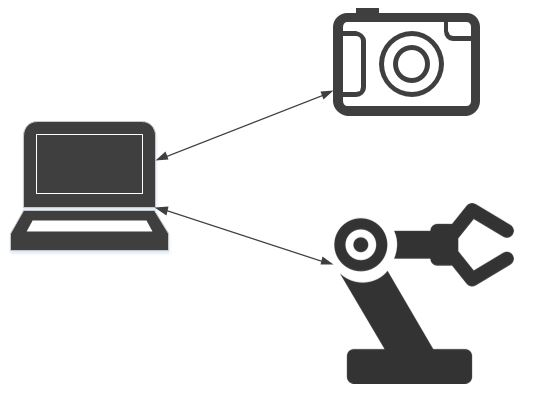
\includegraphics[scale=0.5]{images/hardware}
\caption{Systemoversigt med hardware komponenter}
\label{fig:hardware}
\end{figure}

\subsubsection{Robot} % (fold)
\label{subsub:robot}

\fixme{Ændre 'section' til 'afsnit'}

System anvender en robotarm til at flytte klodserne klodserne fra bordets midte til den side, hvor klodsen er blevet sorteret til. Robotten, som anvendes i systemet, er den i \autoref{sub:crust_crawler} allerede beskrevne AX-12A Smart Robotic Arm fra CrustCrawler Robotics. Robotten styres fra systemets laptop ved at tildele de enkelte joints (rotationsled) en vinkel, som de så indstiller sig til.

% subsubsection robot (end)

\subsubsection{Kamera} % (fold)
\label{subsub:camera}

Systemet anvender et kamera til detektion af klodserne samt vurdering af disses farver. Kameraet, som anvendes i systemet, er et D-Link DCS 930L. Kameraet har en opløsning på $640 \times 480$ pixels og tilsluttes via ethernet. Kameraet er tilsluttet systemets laptop, som henter billeder fra kameraet, når det er nødvendigt.

% subsubsection camera (end)

\subsubsection{Laptop} % (fold)
\label{subsub:laptop}

Systemet anvender en laptop til styring af robotten samt det nødvendige billedbehandling. Denne laptop kører med ubuntu som operativsystem, og har ROS kørende. Systemets laptop er i besidelse af mindst en USB port og ethernet port.

% subsubsection laptop (end)

% subsection hardware (end)
%!TEX root = ../../Master.tex
\subsection{Software} % (fold)
\label{sub:software}

Systemet består ligeledes af et antal softwarekomponenter. I dette afsnit beskrives de forskellige softwarekomponenter og de vigtigste funktioner i disse. Systemets software er skrevet i programmeringssproget Python. \\

%!TEX root = ../../Master.tex
\subsection{Vision system}
Vision systemet består grundlæggende af 4 steps; preprocessering, edge detection, countour detection og til sidst at finde klodserne blandt konturerne. \\

Før udviklingen af vision systemet generede vi et testsæt af billeder og et script til at teste vision systemet på sættet samt at bedømme systemets effektivitet.
Testsættet bestod af 10 billeder taget under forskellige lysforhold og ud fra dem blev der genereret 100 billeder med ændret brightness, contrast og hue. \\

\subsubsection{Preprocessering}


%!TEX root = ../../Master.tex
\subsubsection{Block} % (fold)
\label{subsub:block}

Block er en klasse til håndtering af en klods. Klassen har ansvar for at holde styr på klodsens orientering samt placering i form af et koordinat for klodsens centrum. Dette opnås ved hjælp af klassens to funktioner, som er beskrevet herunder. \\

\textbf{img2base\_transform} \\
Denne funktion har til formål at transformere koordinatsættet fra billedet, som angives i pixels til koordinatsættet for robotten, som angives i cm.\\

Første del af funktionen står for at oversætte pixelkoordinater til koordinater i cm. Dette er gjort ved at finde antallet af pixels på en cm på billedet og derved dele alle pixel koordinater med dette. \\

Den sidste del består i at transformere billedkoordinatsættet til robotkoordinatsættet. De to koordinatsæt er illustret i figur \ref{fig:img2base}, hvor koordinatsættet øverst i venstre side er for billedet og koordinatsættet nederst i midten er for robotten. Som figuren indikerer, kræver denne transformation både translation i x-aksens og y-aksens retning samt en rotation om både x- og z-aksen. \\

\begin{figure}[H]
\centering
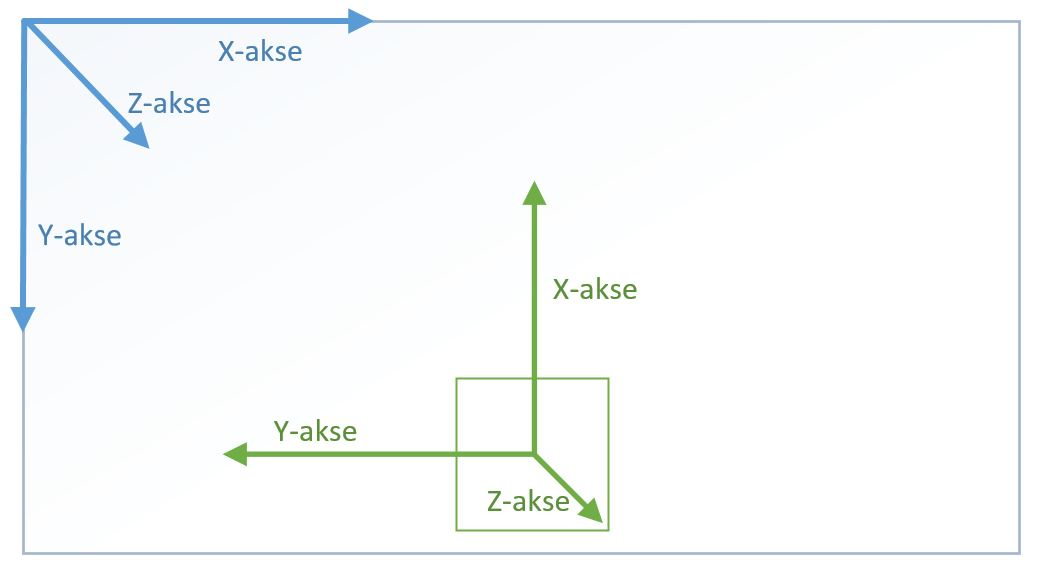
\includegraphics[scale=0.4]{images/img2base}
\caption{Billedkoordinatsæt og robotkoordinatsæt i forhold til bord.}
\label{fig:img2base}
\end{figure}

I implementeringen af dette oprettes derfor to matricer - en transformationsmatrix med både translation og rotation og en rotationsmatrix for den sidste rotation. Dette kan ses i \autoref{transformation}. Matrix A translaterer koordinaterne langs x- og y-aksen og roterer disse omkring x-aksen. Matrix B roterer koordinaterne om z-aksen. For at anvende disse matricer, skal koordinattet, som skal transformeres, være et homogent koordinat.

\begin{lstlisting}[caption=Matricer til transformation., label=transformation, language=Python]
A = np.matrix([
    [1, 0,           0,            tx],
    [0, cos(thetax), -sin(thetax), ty],
    [0, sin(thetax), cos(thetax),  tz],
    [0, 0,           0,            1 ]
    ])

B = np.matrix([
    [cos(thetaz),  sin(thetaz), 0, 0],
    [-sin(thetaz), cos(thetaz), 0, 0],
    [0,            0,           1, 0],
    [0,            0,           0, 1]
    ])
\end{lstlisting}


\textbf{img2joint1\_transform} \\
Denne funktion er en hjælpefunktion, som bruges til at rotere en vektor $[x,y]$ omkring z-aksen. Dette gøres som ved matrix B i \autoref{transformation}. \\


\textbf{find\_orientation} \\
Denne funktion har til formål at bestemme orienteringen på klodsen i forhold til robotten. Klodsen har to orienteringer, da den har to ikke parallelle sider. \\

Fra den tidligere billedprocessering kendes klodsens fire hjørner. Ud fra disse fire hjørner fås to vektorer, som har samme orientering som klodsens to sider. Vinklen mellem hver af disse to vektorer og x-aksen er orienteringen. Vektoren findes ved at trække de to punkter fra hinanden og vinklen opnås ved at bruge tangens på $y/x$. Implementeringen af dette ses i \autoref{orientation}. \\

Den sidste detalje er så, at orienteringen ikke skal regnes ud fra basens x-akse, men i stedet ud fra den x-akse, som følger robottens første rotationsled. Derfor transformeres vektorens koordinater til dette koordinatsystem, som er roteret lige så meget om z-aksen, som robottens første rotationsled, $q1$. Derved kan den beregnede orientation bruges som input til robottens fjerde rotationsled, hvor gripperen er monteret på. \\

\begin{lstlisting}[caption=Funktion til at finde orientering på en klods., label=orientation, language=Python]
def find_orientation(self, q1):
    min_theta = 0

    for i in range(0, 2):
        corner1 = self.img2joint1_transform(self.corners[i][0], self.corners[i][1], q1)
        corner2 = self.img2joint1_transform(self.corners[i+1][0], self.corners[i+1][1], q1)

        dx = corner2[0] - corner1[0]
        dy = corner2[1] - corner1[1]

        theta = atan2(dy, dx)

        if abs(theta) < abs(min_theta) or i == 0:
            min_theta = theta

    return min_theta
\end{lstlisting}
% subsubsection block (end)

%!TEX root = ../../Master.tex
\subsubsection{CrustCrawler}
\label{subsub: CrustCrawler}

Klassen CrustCrawler er en klasse til håndtering af robotarmens positionering. Den har til formål at fortolke det koordinat som fås fra \textbf{block} klassen, og udregne vinkelpositionerne for robotarmens led, således at det er muligt for robotarmen at gribe klodsen.\\

\textbf{inverse\_kinematics\_point}\\
Funktionen har til opgave at udregne og bestemme robotarmens ledvinkler på baggrund af det bestemte midtpunkt for klodserne. Den tager et input (self, x, y, z) som beskriver et punkt for klodserne i rummet, P(x, y, z). Ud fra det bestemte punkt er det muligt at finde positionen til end-effektoren. x, y, z bruges til at beregne $q_1$, $q_2$, $q_3$. Hver q-parameter beskriver en ledvinkel for det tilsvarende led. Udregningen af parametrene kan ses i \autoref{inverse kinematics funktion}\\

Parametrene $r^2, s, D$ er geometriske parametre som anvendes til at bestemme $q_2$ og $q_3$. Nedenfor er det illustreret i \autoref{fig:geometric_approach}, hvordan parametrene tolkes.\\

\begin{figure}[h]
\centering
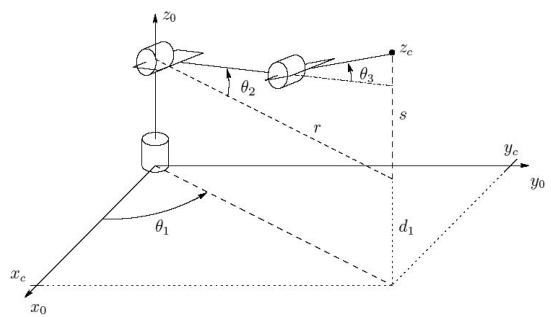
\includegraphics[scale=0.4]{images/geometric_approach}
\caption{Geometrisk bestemmelse af position.}
\label{fig:geometric_approach}
\end{figure}

\newpage
\textbf{inverse\_kinematics\_block}\\
Funktionen har ligesom \textbf{inverse\_kinematics\_point} til opgave at bestemme orienteringen af robotarmensled. Men med fokus på gripperen, så den kan gribe klodsen. Dette sker efter at centrum er fundet. Den kalder funktionen \textbf{find\_orientation} som har fundet den mindste $q_4$-værdi som siger noget om hvor meget gripperen skal roteres i forhold til klodsen.

\begin{lstlisting}[caption=inverse\_kinematics funktion, label=inverse kinematics funktion, language=Python]
    def inverse_kinematics_block(self, x, y, z, block):
        d1 = 10.0  # cm (height of 2nd joint)
        a1 = 0.0   # (distance along "y-axis" to 2nd joint)
        a2 = 20.0  # (distance between 2nd and 3rd joints)
        d4 = 20.0  # (distance from 3rd joint to gripper center - all inclusive, ie. also 4th joint)

        q1 = atan2(y, x)

        # calculation of q2 and q3
        r2 = (x - a1 * cos(q1)) ** 2 + (y - a1 * sin(q1)) ** 2
        s = z - d1
        D = (r2 + s ** 2 - a2 ** 2 - d4 ** 2) / (2 * a2 * d4)

        q3 = atan2(-sqrt(1 - D ** 2), D)

        q2 = atan2(s, sqrt(r2)) - atan2(d4 * sin(q3), a2 + d4 * cos(q3)) - pi / 2

        q4 = - block.find_orientation(q1)

        return q1, q2, q3, q4
\end{lstlisting}

\textbf{move\_to\_point}\\
Funktionen \textbf{move\_to\_point} har til formål generere den sti af punkter som robotarmen skal følge på baggrund af de bestemte positionsværdier i \textbf{inverse\_kinematics\_point}. Den anvender ROS specifikke kommandoer til at bestemme motorerenes position, hastighed og udførselstid. På \autoref{move to point funktion} ses implementeringen af funktionen.\\

Dette foregår altsammen igennem \textbf{JointTrajectoryPoint}, som sætter positionerne til de bestemte værdier i \textbf{inverse\_kinematics\_point} samt begrænsningerne for hvert motorleds acceleration og hastighed. \textbf{JointTrajectory} er ansvarlig for at definere hvilke motorled der indgår i modellen. Sidste del er \textbf{FollowJointTrajectoryGoal} som sætter målet for armen og det afsatte tidsinterval til at nå positionen.\\

\begin{lstlisting}[caption=move\_to\_point funktion, label=move to point funktion, language=Python]
    def move_to_point(self, x, y, z):
        jtp = JointTrajectoryPoint(
            positions=self.inverse_kinematics_point(x, y, z),
            velocities=[0.5] * 4,
            time_from_start=rospy.Duration(2)
        )

        jt = JointTrajectory(
            joint_names=["joint1", "joint2", "joint3", "joint4"],
            points=[jtp]
        )

        goal = FollowJointTrajectoryGoal(trajectory=jt, goal_time_tolerance=rospy.Duration(4))

        self.client.send_goal(goal)
        self.client.wait_for_result()
\end{lstlisting}

\textbf{move\_to\_block}\\
Denne funktion har samme opgave som \textbf{move\_to\_point}, med den ene forskel at dens opgave er at kontrollere motorledene med henblik på klodsorientering.\\

Klassen \textbf{CrustCrawler} har ud over de ovenstående centrale funktioner, underfunktioner som specificerer bevægelsesmønstret for robotarmen i de forskellige situationer ved brug af \textbf{move\_to} og \textbf{gripper} funktionerne. Såsom åbn/luk gripper, saml op/placer klods, placer klods højre/venstre og en reset position.
% subsection software (end)
%!TEX root = ..\Master.tex
\section{Systemarkitektur}

%!TEX root = ..\Master.TEX
\section{Design}
%!TEX root = ..\Master.TEX
\section{Implementering}
%!TEX root = ..\Master.tex
\section{Resultater}
%!TEX root = ../../Master.tex
\clearpage
\section{Diskussion}
Det designede system har vist at det koncept som er forsøgt udviklet er muligt. Systemet er i stand til at tage et billede, registrere objekterne på bordet og afgøre om det er klodser som skal sorteres. Derefter er det i stand til at navigere til centrum af klodsen, rotere sin gripper og samle klodsen op, for derefter at sortere den til den specificerede side.\\

Dog er der i den valgte løsning visse fejlkilder, som kan optræde. Da det er besluttet at der altid startes med at tage et billede af bordet og der derefter foretages billedbehandling betyder det, at systemet er meget følsomt over for ændringer i klods positioner efter billedet er taget. Som en løsning på dette kunne man vælge en løsning, hvor der tages et nyt billede efter hver sorteret klods. Dette vil gøre udførselstiden for opgaven betydeligt længere, men løbende ændringer ville da være mulige at detektere.\\ 

Et andet problem er manglen på check af om klodsen bliver samlet op. For den nuværende implementering vil det betyde at når robotten er færdig med udførslen af sin opgave, retunerer den til udgangspunktet og starter forfra. Det betyder at den vil tage et nyt billede og finde den samme klods, som den så vil forsøge at sortere. Dette problem kan løses på flere forskellige måder. Én måde ville være at anvende en sensor, fx. en tryksensor. På den måde vil systemet få feedback på om den bestemte klods er blevet samlet op. En anden måde ville være at kigge på motorerenes belastning. Da en øget belastning på motorerne må betyde at en klods er blevet samlet op.\\

Der er også observeret fejl i billedbehandlingen. Dette gælder fejl ved sammenligning af farver, som nogen gange gør at to forskellige farver ses som den samme. Det er heller ikke altid at alle klodser detekteres. Dette skyldes at edge detectoren nogle gange laver store huller i den detekterede kant, hvorfor closing transformationen ikke kan lukke hullerne ordentlig, og derfor bliver der ikke tegnet en kontur. Som en løsning på problemet vil det være muligt at indskærme robottens arbejdsområde og tilføre en kendt lyskilde, så belysningen altid er den samme. På den måde opnåes de optimale forhold for at billedet ikke bliver påvirket af udefrakommende faktorer. Dette vil også gøre at hjørneidentificeringen bliver mere præcis og derved er det sikret at de vinkler som bliver fundet i \textbf{block} klassen er de korrekte.\\

Der er en usikkerhed i præcissionen når robotten skal ramme en klods. Dette kan skyldes at koordinatet for klodsen findes på billedets koordinatsæt. Det er valgt at arbejde med at forholdet mellem pixels i billedet og centimeter på bordet er lineært for hele bordet. Hvis en større præcission skulle opnås, ville en bedre kameramodel muligvis kunne hjælpe på dette.\\

Det er set ved brug og test af systemet at robotten har en tendens til at bevæge sig i ryk. Dette kan skyldes at den interne reguleringssløje der styrer motorerne ikke er fintunet til denne specifikke opgave. Det betyder at der er en usikkerhed i robotarmens position. Det ville være muligt at forsøge at fintune den, men det valgt ikke at bruge tid på det da robotten i de fleste tilfælde rammer den bestemte position.\\
%!TEX root = ../../Master.tex
\clearpage
\section{Konklusion}

%----------------------------------------------------------------------------------------
%	REFERENCE LIST
%----------------------------------------------------------------------------------------
\begingroup
	\raggedright
	\bibliography{bibtex/references}
\endgroup

%----------------------------------------------------------------------------------------

\end{document}